\begin{flushright} {\tiny {\color{gray} (tikz\_q1pp02D.tex)}} \end{flushright}
%~~~~~~~~~~~~~~~~~~~~~~~~~~~~~~~~~~~~~~~~~~~~~~~~~~~~~~~~~~~~~~~~~~~~~~~~~~~~~~~~~~~~~~~~~~~~~~~~~~

\begin{center}
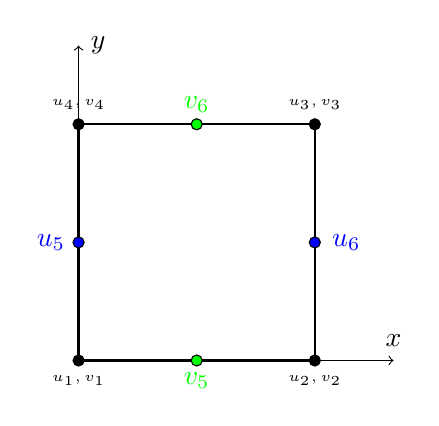
\begin{tikzpicture}
%\draw[fill=gray!23,gray!23](0,0) rectangle (6,5);
%\draw[step=0.5cm,gray,very thin] (0,0) grid (6,5); %background grid

\draw[thick] (1,.5) -- (4,.5) -- (4,3.5) -- (1,3.5) -- cycle; %front

\draw[thin,->] (4,0.5) -- (5,0.5); %x
\draw[thin,->] (1,3.5) -- (1,4.5); %y
\node[] at (5,0.75) {$x$};
\node[] at (1.25,4.5) {$y$};

\draw[black,fill=black] (1,.5)   circle (2pt);
\draw[black,fill=black] (4,.5)   circle (2pt);
\draw[black,fill=black] (4,3.5)   circle (2pt);
\draw[black,fill=black] (1,3.5)   circle (2pt);

\node[] at (1,0.25) {\tiny $u_1,v_1$};
\node[] at (4,0.25) {\tiny $u_2,v_2$};
\node[] at (4,3.75) {\tiny $u_3,v_3$};
\node[] at (1,3.75) {\tiny $u_4,v_4$};

\draw[black,fill=blue] (1,2) circle (2pt); 
\draw[black,fill=blue] (4,2) circle (2pt); 
\node[] at (0.65,2) {\color{blue} $u_5$};
\node[] at (4.4,2) {\color{blue} $u_{6}$};

\draw[black,fill=green] (2.5,0.5) circle (2pt); 
\draw[black,fill=green] (2.5,3.5) circle (2pt); 
\node[] at (2.5,0.25) {\color{green} $v_5$};
\node[] at (2.5,3.75) {\color{green} $v_{6}$};

\end{tikzpicture}\\
\end{center}
